\documentclass{article}
\usepackage[utf8]{inputenc}
\usepackage{geometry}
\usepackage{graphicx}
\usepackage{float}

\usepackage{hyperref}
\hypersetup{
    colorlinks=true,
    linkcolor=blue,
    filecolor=magenta,      
    urlcolor=blue,
}

\geometry{margin=1.5in}
\graphicspath{ {./figures/} }


\title{CSC 751 Project Report: Practical Implementation of OWL Home Ontology}
\author{Katarzyna Pasternak, Zishi Wu}
\date{May 2020}

\begin{document}

\maketitle

%-----------------------------------------------------------------------------
\begin{abstract}
Robotics researchers envision a future in which service robots will assist 
humans  with household tasks. To accomplish this, robotic systems will require
robust decision-making software that can explain its intentions to humans, 
thereby preventing misunderstandings during interactions between humans and 
robots. In this report, we describe the design a prototype
system that combines Natural Language Understanding (NLU) tools with semantic 
triples in order to create explanations on the relative location of household 
items, in a way that is easy for humans to understand. This system is a 
proof-of-concept that Natural Language Understanding and Semantic Web 
technologies can be integrated together to created an Explainable AI 
application that runs on the Toyota Human Support Robot platform.
\end{abstract}

%-----------------------------------------------------------------------------
\section{Introduction}\label{intro}
RoboCup is an annual international robotics competition founded in 1996 with
the aim of promoting robotics and AI research, by offering publicly 
appealing but formidable challenges \cite{RobocupInitiative1996}.
The teams in the RoboCup@Home League are challenged with programming
service robots such as the Toyota Human Support Robot (HSR) \cite{HSR2018} 
(ref. Figure 1) to assist humans with household tasks (e.g. taking out the 
trash). To accomplish these tasks, robots require many capabilities such as 
object detection, object manipulation, navigation, and natural language 
processing. Robots are expected to work with up to 50 different household 
items, including brightly-colored paper bags, cereal bowls, and serving 
trays. The hope is that in the future, service robots will be able to assist 
the elderly and handicapped with household tasks.
\begin{figure}[h]
  \centering
  \begin{minipage}[c]{0.4\textwidth}
    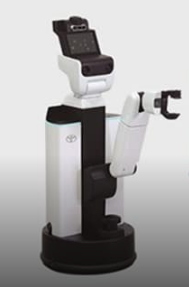
\includegraphics[width=\textwidth]{HSR.png}
    \caption{Human Support Robot by Toyota}
  \end{minipage}
\end{figure}

As it is not feasible to work on all capabilities needed by a robot to 
perform a household task such as taking out the trash, we focused solely on 
the Natural Language Understanding component of the robot. Our end goal was to
design a system that could answer questions regarding the relative location of
household items, and present that information in a natural way similar to how
a human would respond. To accomplish this, we created an home ontology that 
contains household item (e.g. fruit) and household location (e.g. kitchen)
classes and individuals, as well as relationships describing the location
of one object relative to another object 
(e.g. orange \textit{isLocatedInsideOf} fridge).
These household items are a subset of the items specified in the 
\href{http://www.sharelatex.com}{rule book} of the RoboCup@Home League 
\cite{RobocupAtHome2015}.

%-----------------------------------------------------------------------------
\section{Related Work}\label{related}
Bastianelli et al. \cite{BastianelliEtAl2014} used the RoboCup@Home League as
a test-bed for gathering speech corpora in interactions between humans and 
service robots and released their data as a benchmark for spoken language 
interaction in service robotics.

Berners-Lee \cite{bernerslee2001semantic} proposed the idea of a Semantic Web
in which the variations of meaning in human language could be encoded in a 
standardized format for computers, thereby enabling virtual assistants
to understand the nuances in human requests. Hitzler, Krötzsch, and Rudolph
detail the foundations of the Semantic Web technologies, which are rooted in
ontologies and description logics \cite{2009HitzlerBook}. The main advantage
of an ontology lays in its ability to explain how a software program reached
its decision, a phenomena known as \textit{Explainable AI} or \textbf{XAI}
for short. Anjomshoae et al. \cite{AnjomshoaeEtAl2019} define Explainable AI
as a domain ``aiming at building explainable agents and robots capable of 
explaining their behavior to a lay user.'' In this project, we propose to 
combine ontologies and the RoboCup@Home League challenges to create an 
Explainable AI system that can enable service robots to explain the location 
of household items in a way that is natural to humans.

\subsection{Semantic Triples}
To accomplish this, we used semantic triples to encode information regarding
the relative location of household items. A \textit{semantic triple} is a set 
of three entities --- subject, predicate, object --- 
that form a statement about the world. For example, in the statement 
``Plato is a student of Socrates'', the subject is \textit{Plato}, the 
predicate is \textit{is a student of}, and the object is \textit{Socrates}.
Note that the predicate is also referred to as the relationship.

We encoded the relative location of a set of household items into semantic 
triples. The set of subjects included \textit{orange, banana, mustard, 
ketchup}, and \textit{bowl}. The set of objects included \textit{fridge,
table}, and \textit{chair}. Finally, the set of predicates consisted 
of five relative location descriptions: \textit{is located on top of}, 
\textit{is located below}, \textit{is located to left of}, 
\textit{is located to right of}, \textit{is located inside}. 

The statement, ``the bowl is on top of the kitchen table'' is an 
example of a fully formed semantic triple that our system can generate as a 
response to the question, ``where is the cereal bowl?'' The statement has no 
ambiguity and the user interacting with the system can quickly go to their 
refrigerator to check. In contrast, a robotic system that does not have a 
Natural Language Understanding module that leverages semantic triples may 
instead respond with raw spatial information from a 2D image. In that
scenario, the robot may respond by saying,
``the cereal bowl is bounded by pixel coordinates (10, 10), (20, 10), 
(10, 40), (20, 40) and the kitchen table is bounded by coordinates (0, 40), 
(100, 40), (0, 80), (100, 80)''. The advantage of using semantic triples is 
that humans find it much easier to understand information on relative 
location when it is presented in the form of triples, as opposed to raw 
coordinate data.

\subsection{Assumptions}
To narrow the scope of the project, we made the following assumptions:
\begin{itemize}
    \item The robot has already detected the household objects and mapped 
        their locations.
    \item There is already a script that converts the robot's mapping and
        object detection data into relative location data.
\end{itemize}
Under these assumptions, we encoded information on the relative location of
household items as semantic triples into an ontology in the home domain.

%-----------------------------------------------------------------------------
\section{Design of System}

The system is divided into two parts: a front-end written in Python that 
handles natural language understanding and user interaction tasks, and a 
back-end written in Java that queries the ontology for the location of an
object. 

\subsection{Front-End}
First, the Python front-end of the program introduces itself as 
\textit{Palpi}, the name given to the Toyota Human Support Robot that it runs 
on. It then prompts the 
user by asking if they would like to know the location of an item. The user 
can respond with a question such as ``Where is the orange?'' A microphone 
module listens for questions. If the program does not hear a question after 
about 10 to 15 seconds, it will say ``Sorry, I couldn't hear that.'' and 
prompt the user again. If the program does hear a question, it will send an 
audio recording to the Google Cloud Speech-to-Text API and get back a text 
transcript.

The text is then processed by Rasa, an open-source natural language 
understanding library for handling tasks such as entity and intent 
recognition \cite{bocklisch2017rasa}. Rasa uses Tensorflow to train a neural 
network model on thousands of sentence examples. These sentences are 
generated by using Chatito, a domain-specific language that allows the user 
to generate training examples for natural language understanding tasks. In 
Chatito, users specify a grammar that the training examples generated should 
follow, with slots for interchangeable words.
For example, in the question ``where is the orange'', the word \textit{orange}
can be interchanged with \textit{mandarin} or \textit{citrus}. Thus in 
Chatito we would specify in the grammar that the last word in the sentence
is a slot with three possibilities: orange, mandarin, and citrus. Chatito 
also allows us to specify which words refer to entities and which refer to
intentions. For example, the word \textit{where} refers to an intention 
(e.g. inquiry into the location of something) while the word \textit{orange}
refers to an entity (e.g. the object that we wish to know the location of).
After it is trained on sentence examples generated by Chatito, Rasa can 
recognize the entity and intention keywords in a sentence.

\subsection{Back-End}
The keywords recognized by Rasa are sent to a back-end module written in Java 
that serves as an interface between the user's questions and the home 
ontology. The back-end module uses the recognized entities and intentions to 
build a query in the SPARQL Protocol and RDF Query Language, or SPARQL for 
short. For example, when a user asks the question ``where is the orange'', 
Rasa will recognize an entity named \textit{orange} and a \textit{location} 
intention from the \textit{where} keyword. The back-end Java module then generates a SPARQL query from these keywords that selects all the triples 
where the subject is an orange and the predicate is a type of location 
relationship (e.g. \textit{isLocatedInside}).

To test our system, we created several individuals in the ontology, 
including two individuals named \textit{orange} and \textit{fridge}.
We defined a semantic triple ``orange \textit{isLocatedInside} fridge'', 
which is returned as a result from executing the SPARQL query and then 
written to a text file. The front-end then converts this into a more natural 
format, ``orange is located inside the fridge.'' Finally, the front-end
uses the Google Cloud Text-to-Speech API to convert the text transcript into 
audio and play the audio response back to the user.

If the SPARQL query failed to find a matching triple in the ontology, then
the program will notify the user by saying, ``Sorry, I don't know the 
location of this object.'' If the SPARQL query finds multiple matching 
triples in the ontology, then the program will say the triples, one by one.
For example, if the user asks, ``where is the fruit,'' the program first says
``orange is located inside of fridge,'' and then says, 
``banana is located on top of table.''

\subsection{System Outline}
Outlined below is a list of steps that details how the program runs:
\begin{enumerate}
    \item The user says a question to the program: ``where is the orange?"
    \item The program sends an audio file to the Google Cloud Speech-to-Text 
        service and receives back a text transcript: ``where is the orange?''
    \item The program passes the text transcription through Rasa's intent     
        parser to extract entity and intention keywords.
    \item The program checks if the entity (e.g. orange) and intention
        (e.g. location of) keywords exist in the ontology.
    \item If the keywords exist in the ontology, the program runs
        steps 6 through 10. If they don't exist, the program goes to step 11.
    \item The program uses the entity and intention keywords to build a 
        SQARQL query and executes it.
    \item The SPARQL query looks for all triples where the subject is             an \textit{orange} and the predicate is a sub-class of the 
        relationship class \textit{isLocationOf}. Sub-class relationships
        in this case include: \textit{isLocatedOnTopOf}, 
        \textit{isLocatedBelow}, \textit{isLocatedToLeftOf}, \textit{isLocatedToRightOf}, \textit{isLocatedInside}.
    \item The SPARQL query returns semantic triples that match:
        \textit{orange isInsideOf fridge}.
    \item The program converts the results of the query into a more 
        natural sentence: ``orange is located inside of fridge''.
    \item The program passes the response text to the 
        Google Text-to-Speech service and gets back an audio file. It plays
        the audio file, which consists of synthesized speech audio.
    \item The program responds by telling the user that the entity they are 
        looking for does not exist in the ontology.
    \item Part (a). The program asks the user about the properties of the     
        entity, starting with whether or not the entity belongs to any of the 
        base classes of the ontology (Food, CleaningItem, Furniture). It 
        filters out the individuals that do not belong to that class and then 
        repeats the question, this time with a sub-class of the base class. 
        This exchange continues until the necessary information is collected 
        (i.e. we arrive at a class with no sub-class). 
        
        Part (b). The program ends up with an individual $Y$ in the ontology 
        that belongs to the same class $C$ as the individual $X$ that the 
        user inquired of. It then informs user that while it does not know
        the location $Y$, it found an object $X$ that belongs to the same
        class as $Y$ and suggests that $X$ might be in the same location 
        as $Y$.
\end{enumerate}

\begin{figure}[!h]
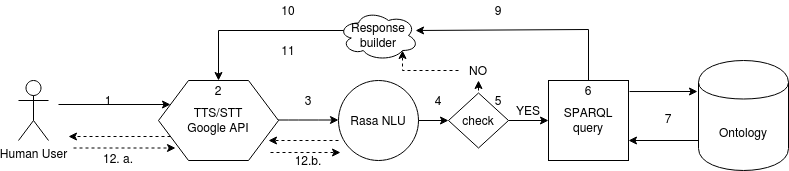
\includegraphics[width=\textwidth]{system_diagram.png}
\end{figure}

\subsection{Limitations}
Due to time constraints, we were unable to implement the features 
described in parts 12 (a) and 12 (b) of the system diagram. We were only able
to get the program working for the case where the item does exist in the 
ontology. If the item does not exist in the ontology, the program simply 
replies that the item does not exist and asks the user if they would like to 
ask another question.

%-----------------------------------------------------------------------------
\section{Dependencies}
The following is a list of software tools we used in this project.
\begin{itemize}
    \item Robot Operating System (ROS), Kinetic version: 
        http://wiki.ros.org/kinetic/Installation
    \item Ontology Web Language (OWL) API: https://github.com/owlcs/owlapi
    \item Apache Jena: https://jena.apache.org/
    \item Protege: https://protege.stanford.edu/
    \item Rasa NLU: https://github.com/RasaHQ/rasa
    \item Google Cloud Speech-to-Text API: 
        https://cloud.google.com/speech-to-text/
    \item Google Cloud Text-to-Speech API: 
        https://cloud.google.com/text-to-speech/
    \item Chatito: https://github.com/rodrigopivi/Chatito
    \item Python 2 Speech Recognition API: 
        https://pypi.org/project/SpeechRecognition/
\end{itemize}

ROS is a set of middleware libraries for robots. It enables users to develop 
reusable packages and services to handle specific tasks in robotics such as
speech recognition, navigation, and mapping. ROS is widely used in both
academia and industy, and can operate on various robotics platforms. 
For this project, we developed a package that allows users to ask a robot 
questions about the location of an item in a house. 

The Ontology Web Language (OWL) API is a Java library for manipulating 
ontology files. We used Apache Jena to convert OWL ontology files into an 
RDF data format that can then be queried on by SPARQL queries.
To rapidly prototype and test SPARQL queries, we used Protege, an application
for creating and validating ontologies. 

To convert user questions from speech to text and the program's responses 
from text to speech, we used services provided by Google Cloud. Chatito was
used to generate training examples of questions that the program might expect
to hear from users, and the Python 2 Speech Recognition API was used to 
enable the program to ``listen'' for the user's questions. The reason why we
used Python 2 instead of Python 3, even though Python 2 is no longer being 
updated as of 2020, is because we are using an older version of ROS called 
ROS Kinetic, which is written using a mix of C++ and Python 2.

\newpage

%-----------------------------------------------------------------------------
\section{Results}
At the base of our project, we used the following house ontology:
\begin{figure}[H]
\centering
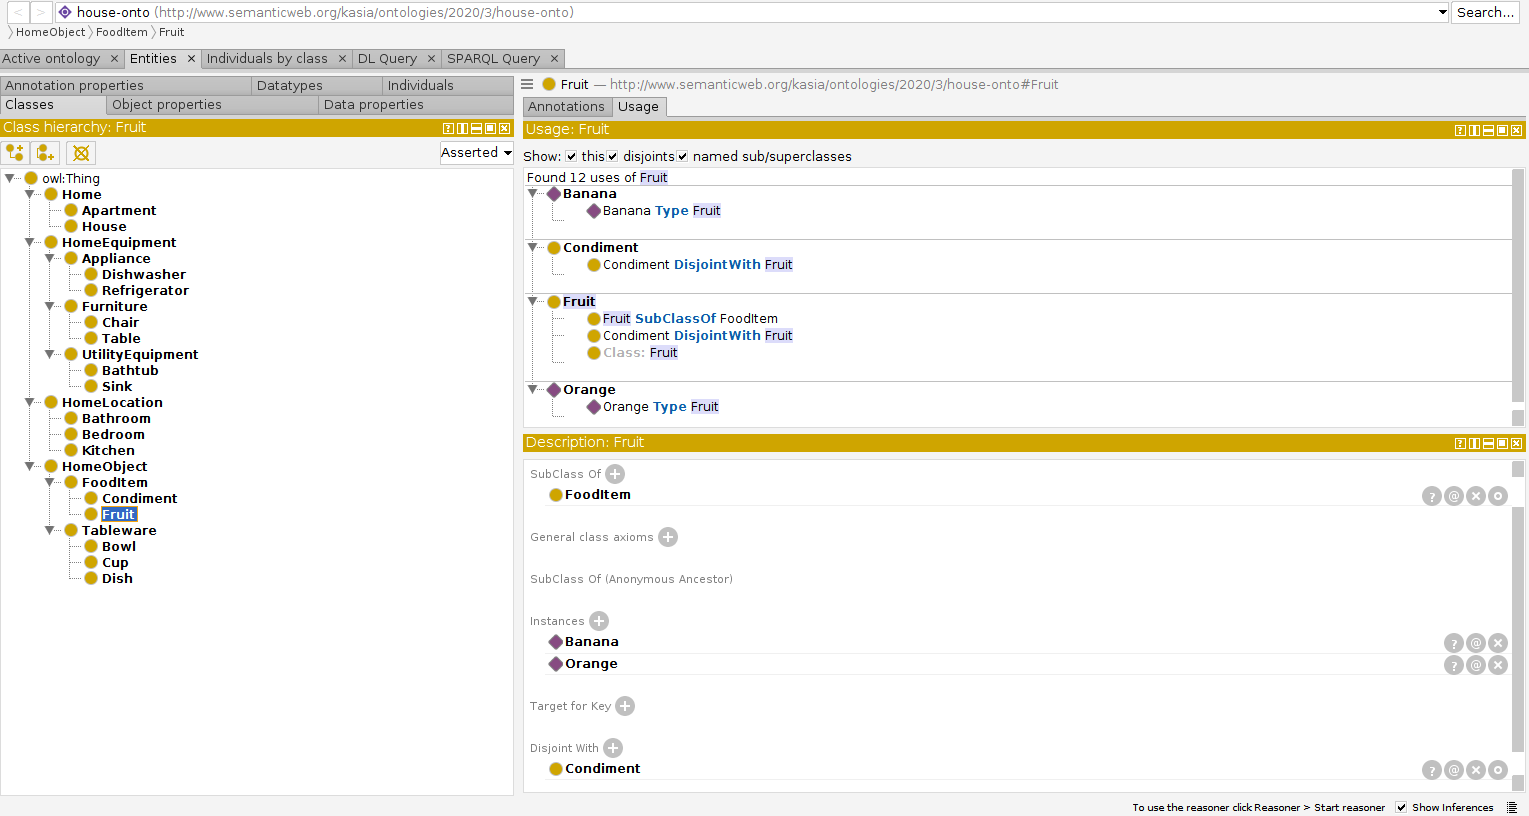
\includegraphics[width=\textwidth]{onto_protege.png}
\end{figure}

When running our program, the user observing the terminal can see the 
following process. First, the user can run the program with the command:
\begin{figure}[H]
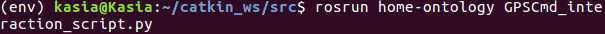
\includegraphics[width=\textwidth]{run_code.png}
\end{figure}

Next, the robot (or the computer running the program) initiates the 
conversation with the user by introducing itself as ``Palpi'' and the user
what household items they would like the robot to find.
\begin{figure}[H]
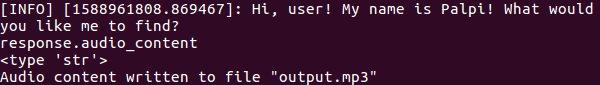
\includegraphics[width=\textwidth]{start.png}
\end{figure}

Then program listens to the user speech and finds the entity and intention
keywords. In this case, the intention is \textit{find} and the entity is
\textit{fruit}.
\begin{figure}[H]
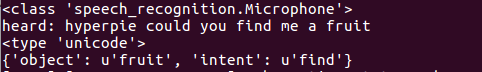
\includegraphics[width=\textwidth]{find.png}
\end{figure}

Then the program executes a SPARQL query on the ontology ontology for given 
entity and intention pair, and writes the resulting semantic triple(s) in an
output file. The output is read from the file, formatted, and synthesized 
into an audio file that is spoken to the user.
\begin{figure}[H]
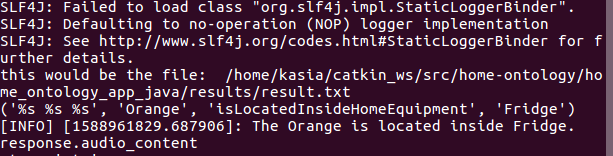
\includegraphics[width=\textwidth]{query.png}
\end{figure}

Finally, the robot (our machine) asks if there is anything else to find. If 
the answer is ``yes,'' then the program repeats the whole process again.
If the answer is ``no'', then the program finishes executing.
\begin{figure}[H]

\includegraphics[width=\textwidth]{loop.png}
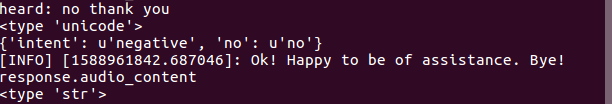
\includegraphics[width=\textwidth]{no.png}
\end{figure}

%-----------------------------------------------------------------------------
\section{Future Work}
When encountering instances of household items that the ontology has no 
prior information of, the program currently says ``sorry, I don't know the 
location of that object'' and asks the user if they would like to ask another
question. In future work, we would like to make the robot more pro-active by
programming it to ask the users about the properties of the item that does not
exist in the ontology, and and try to infer the location of the item based on 
other items that fall in the same category. For example, suppose that the 
ontology contains the following information
\begin{itemize}
    \item $\{$milk, cranberry juice$\}$ $\in ($LiquidFood $\cup$ ColdFood$)$
    \item $\{$milk, cranberry juice$\}$ $isLocatedInsideOf$ fridge
    \item $\{$LiquidFood, SolidFood, ColdFood, WarmFood$\}$ $\subset$ Food
\end{itemize}

Now suppose the following conversation occurs, where $P$ denotes a person
speaking and $R$ denotes the robot speaking. Furthermore, suppose the ontology
does not contain information on an individual named \textit{orange juice}.
\begin{itemize}
    \item P: ``Where is the orange juice?''
    \item R: ``I'm not sure but can you tell me about the orange juice?''
        (Behind the scenes the robot builds a starter question based on the
        basic classes of the household item ontology; suppose they are:
        Food, CleaningItem, and Furniture).
    \item R: ``Is orange juice a type of food, cleaning item, or
        furniture?''
    \item P: ``Orange juice is a type of food.'' (The robot can ask a new 
        question based on the sub-classes of Food).
    \item R: ``Is orange juice a type of cold food or warm food?''
    \item P: Cold food. (The robot rules out instances in the ontology that
        are not a type of ColdFood).
    \item R: ``Is orange juice a type of liquid food or solid food?''
    \item P: Liquid food. (The robot rules out instances in the ontology
        that are not a type of LiquidFood).
    \item R: ``I'm not sure where the orange juice is, but I think it might
        be in the refrigerator.''
    \item P: ``Why?''
    \item R: ``Well, orange juice is a type of liquid food and cold food.
        It so happens that milk and cranberry juice also fall into both 
        these categories, and they are located in the refrigerator.''
\end{itemize}

By using Semantic Web technologies and inference methods, we can give a
robot the ability to make an educated guess regarding the location of an
item it has not previously detected. In addition to this, Semantic Web 
technologies enable a robot to explain to a user the reasoning behind why it
decided on such a guess. This is all presented in the form of semantic 
triples, which can encode information on relative location in a format that
is easy for humans to understand.

%-----------------------------------------------------------------------------
\section{Conclusion}
In this paper, we presented the design of a prototype system that combines 
natural language understanding with semantic web triples that answers 
inquires regarding the relative location of common household items in a clear
manner that resembles how humans expect spatial information to be presented.
In the future, we plan to extend this technology to handle cases where the 
ontology does not have information regarding an entity but uses inference
rules to suggest the most likely location based on class similarity between
entities. As demonstrated, systems containing Explainable AI modules show
great promise in service robot applications due to the fact that when asked
about their reasoning for a decision, such systems can provide a clear answers
in the form of semantic triples. As virtual software and physical robotic 
assistants are developed for more complex decision-making processes, systems
that incorporate Explainable AI will become critical to ensuring safety for
humans interacting with robots.

\bibliographystyle{unsrt}
\bibliography{references}

\end{document}
